\documentclass[UTF8]{article}
% Template based on https://www.overleaf.com/latex/templates/assignment-template/fwycphfzpshm

\usepackage[authoryear]{natbib}
\usepackage{url}
\usepackage{amsmath}
\usepackage{amsfonts}
\usepackage[margin=1in]{geometry}
\usepackage{multirow}
\usepackage{graphicx}
\usepackage{pdfpages}

\title{AttentiveCLS Pooler}
\author{
  Team 1:  % team no
  Seungil Lee, Jongchan Park, Eugene Seo, and Dohyung Kim % your names
}
\date{\today}

\begin{document}
\maketitle

\section{Introduction}

BERT~\cite{devlin-etal-2019-bert} has become a standard architecture for NLP research ever since it was published. BERT computes the representation for every token, but it uses the output representation of the special token \texttt{[CLS]}, for sentence-level tasks (e.g., sentiment analysis). However, various strategies were introduced to get sentence-level representation.

We have designed a new pooler named \texttt{AttentiveCLS} pooler and evaluated its performance on CoLA, MNLI, RTE and SST-2 tasks, which are the representatives of sentence-level tasks. The results were compared with \texttt{MeanMaxTokens} pooler, which is suggested in the homework description, also with the original \texttt{BERTPooler} in \texttt{huggingface} library (\url{https://huggingface.co/}).

\section{AttentiveCLS Pooler}
Though the original BERT pooler simply adopts the last output of \texttt{[CLS]} token, we tried to exploit information from other tokens as well. Nowadays, an attention mechanism is widely used to get the importance of the given sequence, so we added an attention pooling layer on the top of the tokens other than \texttt{[CLS]} token. Then, the output of this attention layer is concatenated with the last output of \texttt{[CLS]} token. We also applied linear transformation with $W \in \mathbb{R}^{H \times 2H}$ and $\tanh$ activation just like as the \texttt{BERTPooler} in \texttt{huggingface} implementation.

\begin{figure}[htp] \centering{
  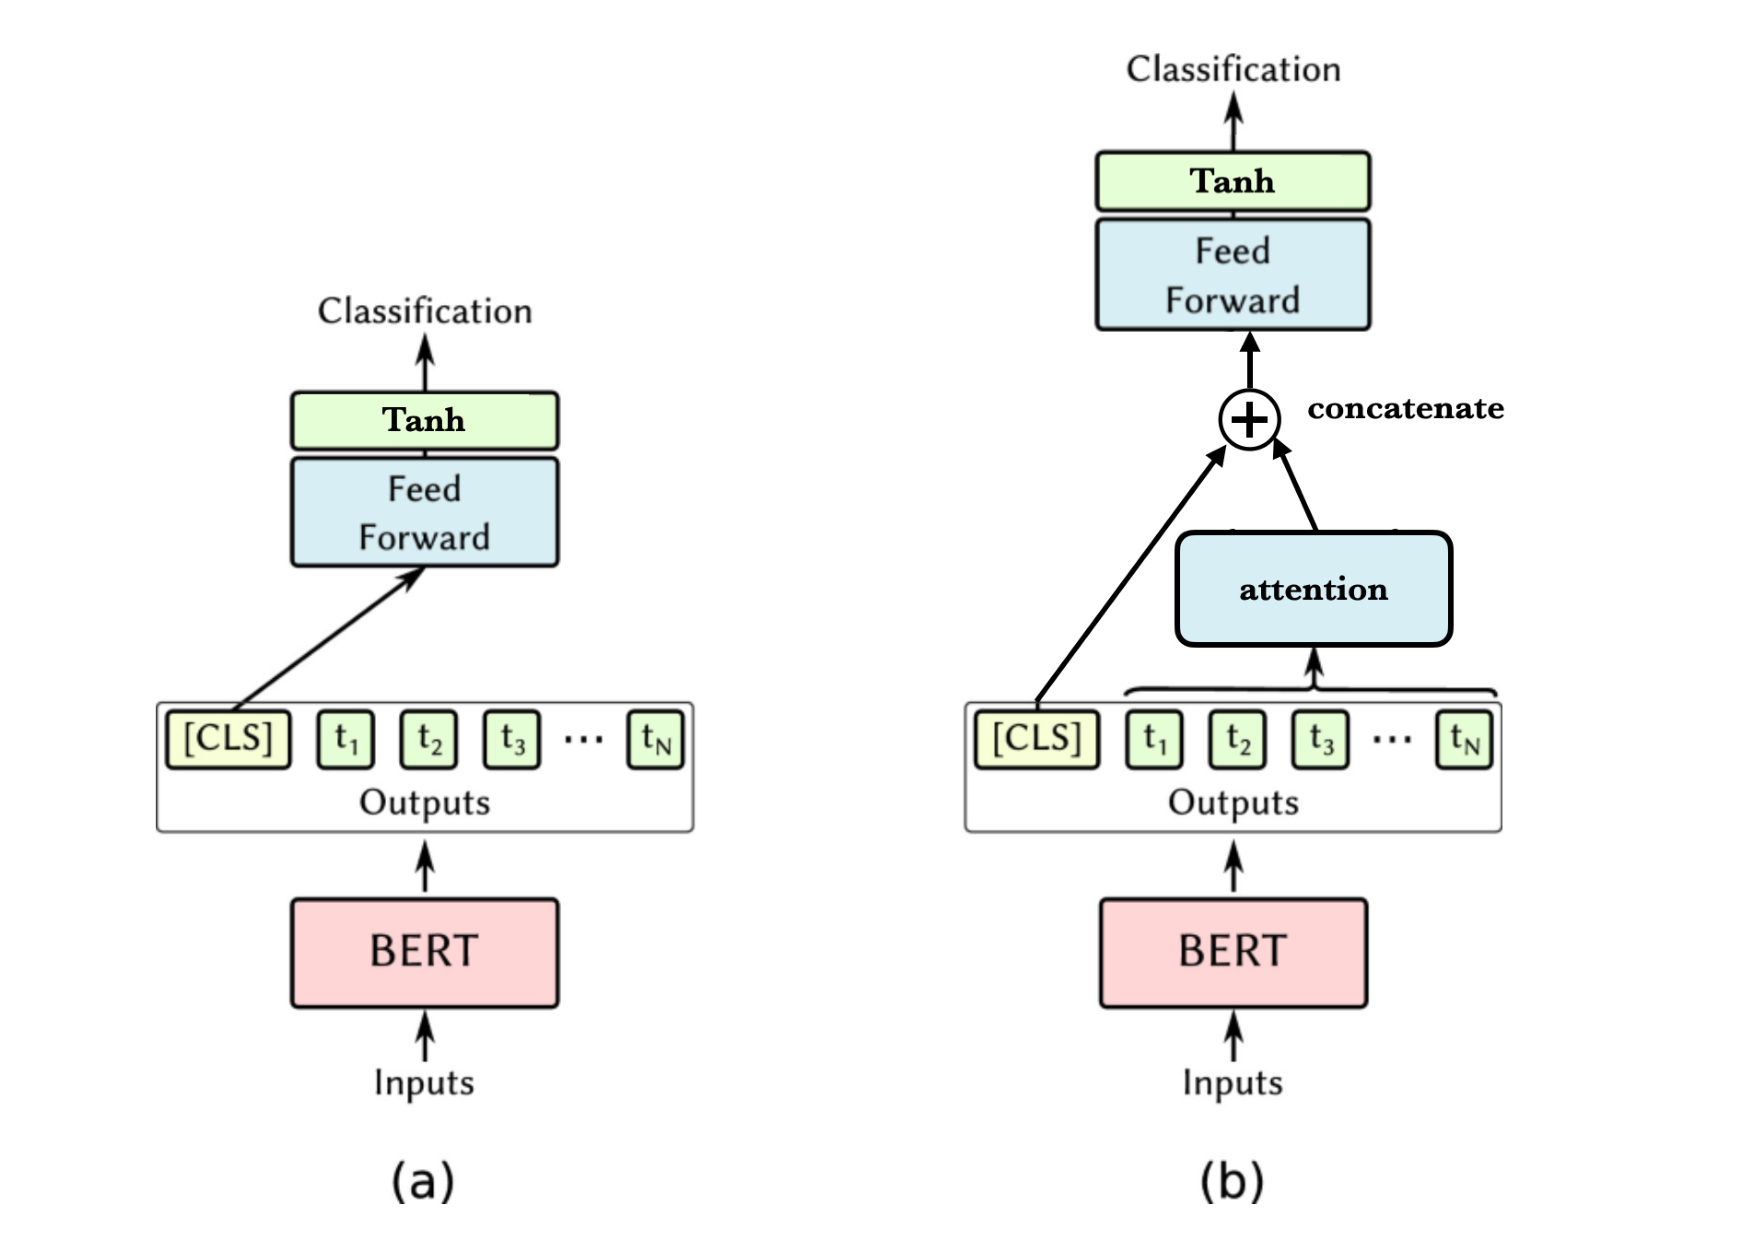
\includegraphics[scale=0.4]{figure1.pdf}}
  \caption{Schematic visualization of AttentiveCLS. This figure is modified from the paper~\cite{lehevcka2020adjusting}.}
  \end{figure} 


\section{Result}

\begin{table}[]
\resizebox{\textwidth}{!}{%
\begin{tabular}{|l|ll|lll|ll|ll|}
\hline
\multirow{2}{*}{} & \multicolumn{2}{l|}{CoLA}                                   & \multicolumn{3}{l|}{MRPC}                                                                     & \multicolumn{2}{l|}{RTE}                               & \multicolumn{2}{l|}{SST-2}                             \\ \cline{2-10}
& \multicolumn{1}{l|}{Loss}            & Matthews & \multicolumn{1}{l|}{Accuracy}        & \multicolumn{1}{l|}{F1}              & Loss            & \multicolumn{1}{l|}{Accuracy}        & Loss            & \multicolumn{1}{l|}{Accuracy}        & Loss            \\ \hline
AttentiveCLS      & \multicolumn{1}{l|}{0.4588}          & 0.6044               & \multicolumn{1}{l|}{\textbf{0.8544}} & \multicolumn{1}{l|}{\textbf{0.9012}} & \textbf{0.3952} & \multicolumn{1}{l|}{0.6137}          & 0.7498          & \multicolumn{1}{l|}{0.9289}          & 0.3272          \\ \hline
MeanMax           & \multicolumn{1}{l|}{\textbf{0.4246}} & \textbf{0.6060}      & \multicolumn{1}{l|}{0.8382}          & \multicolumn{1}{l|}{0.8907}          & 0.4570          & \multicolumn{1}{l|}{0.6101}          & \textbf{0.6818} & \multicolumn{1}{l|}{\textbf{0.9300}} & \textbf{0.2206} \\ \hline
BERTPooler        & \multicolumn{1}{l|}{0.4388}          & 0.5934               & \multicolumn{1}{l|}{0.8456}          & \multicolumn{1}{l|}{0.8934}          & 0.4000          & \multicolumn{1}{l|}{\textbf{0.6462}} & 0.7058          & \multicolumn{1}{l|}{\textbf{0.9300}} & 0.2387          \\ \hline
\end{tabular}%
}
\caption{Table showing the result of 4 experiments. Bold numbers indicate the best performance among 3 poolers.}
\label{tab:result}
\end{table}

In this experiment, 4 different text classification tasks (CoLA, MRPC, RTE, SST-2) in the GLUE~\cite{wang2018glue} benchmark were chosen to evaluate 3 pooling strategies. Each dataset has its own evaluation metrics (e.g. Accuracy, F1).

Table \ref{tab:result} shows our experiment results. 
\begin{enumerate}
    \item CoLA: \texttt{MeanMax} reached the highest performance in terms of Matthews correlation score and validation loss. \texttt{AttentiveCLS} beated \texttt{BERTPooler}.
    \item MRPC: Interestingly, \texttt{AttentiveCLS} was superior to other strategies in terms of all evaluation metrics.
    \item RTE: \texttt{AttentiveCLS} did not perform better than others. \texttt{BERTPooler} had the best accuracy and \texttt{MeanMax} had the lowest loss. 
    \item SST-2: Both \texttt{MeanMax} and \texttt{BERTPooler} showed the best accuracy and \texttt{BERTPooler} had the best loss value.
\end{enumerate}

This result showed that each pooler can make different performances depending on the dataset. 
\texttt{AttentiveCLS} took a first place in MRPC, while it was not performed well in CoLA, RTE and SST-2. However, the differences were insignificant. There was no big difference in performance according to the pooler, so we concluded that the pooler strategy had no critical effect on text classification task.


\bibliographystyle{plain}
\bibliography{report.bib}


\end{document}
